\section{The Method of Green's Functions}
\setcounter{example}{0}
\subsection{Introduction}
A \df{Green's function} is the solution to a differential equation of the form
\begin{equation} \label{eq:greensdef}
    \opp{L^*_\xi} G(\xi, x) = \delta(\xi - x). 
\end{equation}
The subscript \(\xi\) on the differential operator indicates that the derivatives are being taken with respect to the variable \(\xi\). By making use of some of the delta function's unusual properties, Green's functions can be used to solve nonhomogeneous linear differential equations.

To find the solution to the linear differential equation
\begin{equation} \label{eq:4.2}
    \opp{L}u=\phi,
\end{equation}
we start by finding the formal adjoint as in equation (\ref{eq:adjoint}). If we replace \(v\) with \(G\), and we replace \(x\) with a dummy variable \(\xi\), we are left with an equation of the form
\begin{equation} \label{eq:greenadjoint}
    \intl G(\xi, x)\opp{L}u(\xi) d\xi = \bterms + \intl u(\xi)\opp{L^*}G(\xi,x) d\xi.
\end{equation} 
It follows from equation (\ref{eq:greensdef}) that we can replace \(\opp{L^*}G\) with \(\d\), and from equation (\ref{eq:4.2}) that we can replace \(\opp{L}u\) with \(\phi\), 
\begin{equation}
    \begin{split}
        \intl G(\xi,x)\phi(\xi) d\xi &= \bterms + \intl u(\xi)\d(\xi-x) d\xi\\
        &=\bterms + u(x).
    \end{split}
\end{equation}
Therefore, if we choose boundary conditions for \(G\) such that the boundary terms do not depend on \(u\) and we are able to find \(G\), then finding \(u\) is reduced to a problem of integrating \(G\phi\). 

To illustrate the key ideas of the method, we will consider several examples which begin simply and become more complex. Each example will be concerned with a key concept in implementing the method of Green's functions.

\subsection{Example 1 \textit{ Loaded String}}
    
    Consider the boundary value problem
    \begin{equation} \label{ex1:initialize}
        u''(x) = \phi(x);\quad u(0)=u(1)=0
    \end{equation}
    where \(\phi(x)\) is prescribed. Equation (\ref{ex1:initialize}) can be regarded as describing the static deflection of a string under unit tension between fixed endpoints and subjected to a force distribution \(\phi(x)\).

    \begin{figure}\label{fig:LoadedString}
    \centering
    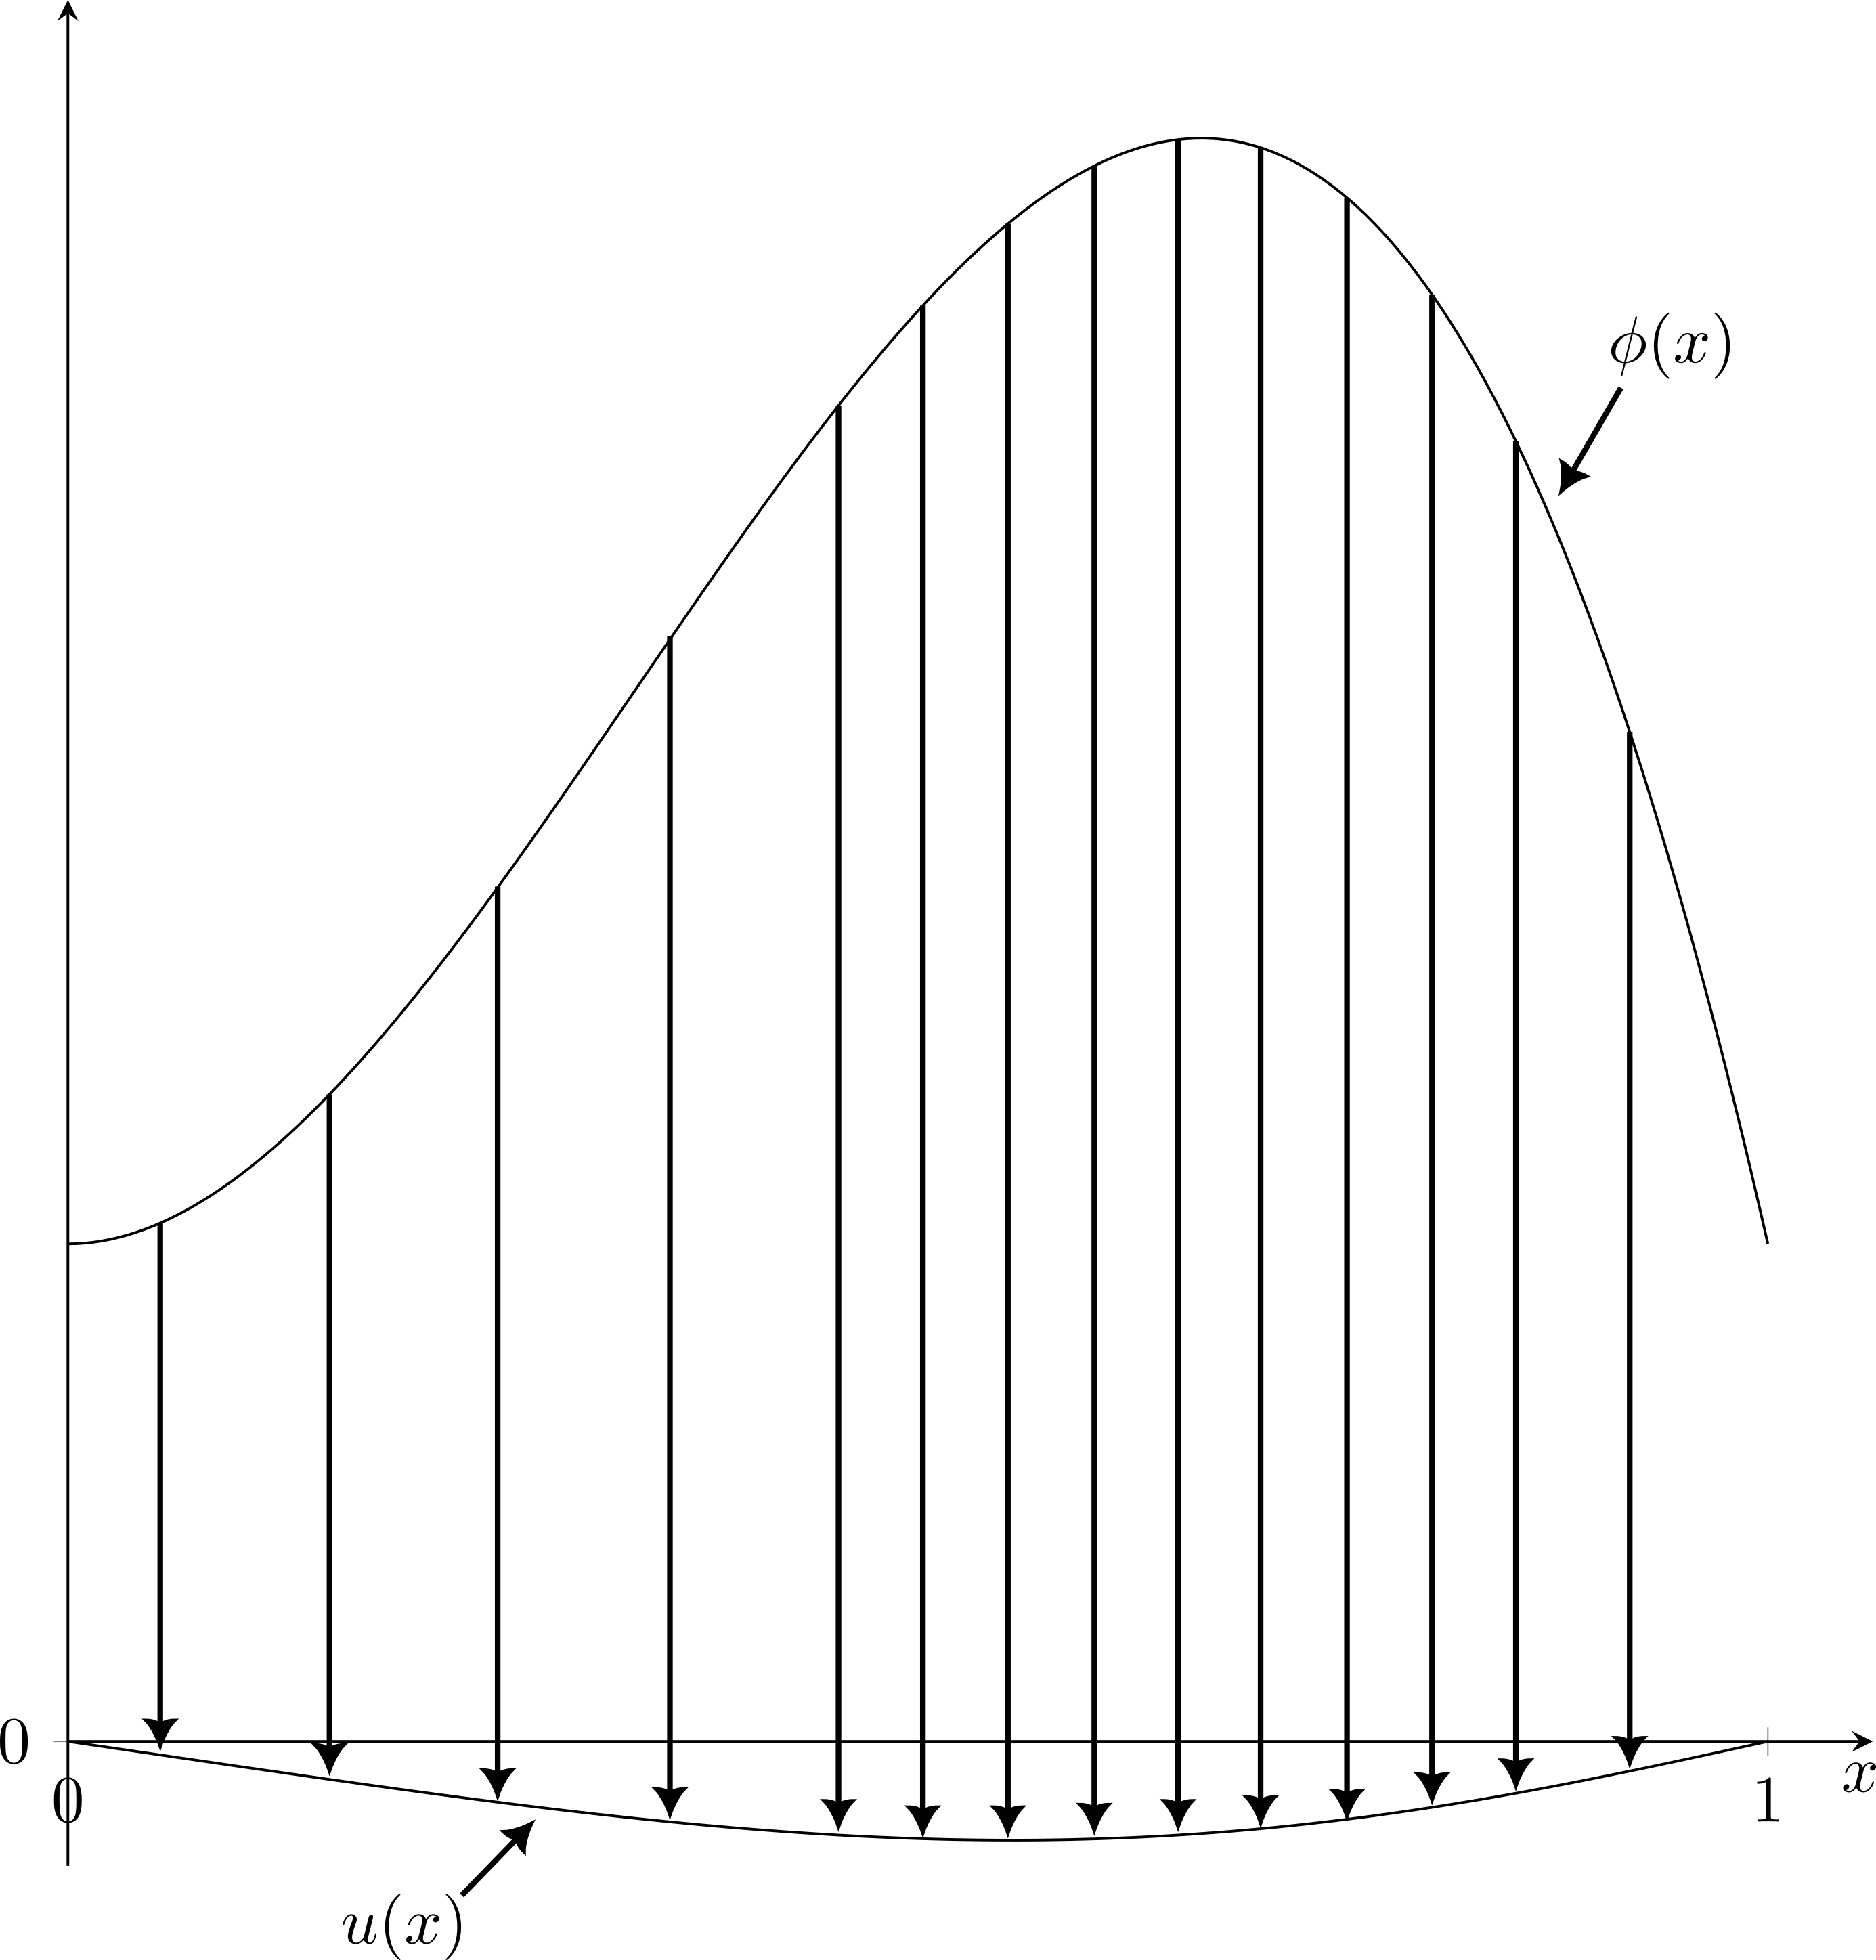
\includegraphics[width=0.5\linewidth]{include/loadedstring.png}
    \caption{Loaded String}
\end{figure}
    
    To find a solution to this differential equation, we first find the formal adjoint \(\L*\) as in equation (\ref{eq:greenadjoint}). 
    \begin{equation}
        \begin{split}
            \int_{0}^{1} G(\xi, x)\L u(\xi) d\xi  &= (G(\xi, x)u'(\xi)-G_\xi (\xi, x)u(\xi))\biggr\rvert_0^1 + \int_{0}^{1} uG_{\xi\xi}d\xi\\
            &= G(1, x)u'(1) - G_\xi(1, x)u(1) \\&- G(0, x)u'(0) + G_\xi(0,x)u(0) + \int_{0}^{1} uG_{\xi\xi}d\xi.
        \end{split}
    \end{equation}
    Therefore, 
    \begin{equation}
        \Lstar = \frac{d^2}{d\xi^2}
    \end{equation}
    and 
    \begin{equation}\label{eq:loadedStringLstarG}
        \Lstar G = G_{\xi\xi} = \delta(\xi-x).
    \end{equation}
    Because of the boundary conditions on \(u\) in equation (\ref{ex1:initialize}), two of our boundary terms are zero. Thus,
    \begin{equation}
        \int_{0}^{1} G(\xi, x)\L u(\xi) d\xi = G(1, x)u'(1) - G(0, x)u'(0) + \int_{0}^{1} uG_{\xi\xi}d\xi.
    \end{equation}
    Now, we want to remove the \(u\) dependency from the boundary terms and, as such, decide that
    \begin{equation}
        G(1,x) = G(0,x) = 0.
    \end{equation}
    Then the solution is given by 
    \begin{equation}\label{eq:loadSln}
        u(x) = \int_0^1 G(\xi,x)\phi(\xi)d\xi.
    \end{equation}
    To calculate the Green's function, we integrate equation (\ref{eq:loadedStringLstarG}), regarding \(x\) as fixed.
    \begin{equation}
        \begin{split}
            G_\xi &= H(\xi-x) + A\\
            G &= (\xi - x)H(\xi-x)+A\xi +B
        \end{split}
    \end{equation}
    Imposing the boundary conditions, 
    \begin{equation}
        \begin{split}
            &G(0,x) = 0 = B\\
            &G(1,x) = 0 =  1 - x + A + B,
        \end{split}
    \end{equation}
    shows us that \(B=0\) and  \(A=x-1\). Therefore
    \begin{equation}
        G(\xi,x) = (\xi-x)H(\xi-x) + (x-1)\xi.
    \end{equation}

    Equation (\ref{eq:loadedStringLstarG}) can, like equation (\ref{ex1:initialize}), be interpreted as the deflection of a loaded string. Specifically, it is the deflection as a function of \(\xi\) due to a point load of unit strength, \(\d(\xi-x)\), instead of a load distribution, \(\phi\). Rewriting our Green's function as
    \begin{equation}
        G(\xi,x)= \begin{cases}
            (x-1)\xi, & \xi \leq x\\
            (\xi-1)x, & \xi \geq x
        \end{cases}
    \end{equation}
    makes it clear that \(G(\xi,x)\) is symemtric, to wit: \(G(\xi,x)=G(x,\xi)\). This is often referred to as "Maxwell Reciprocity." Because of this reciprocity, \(G(\xi,x)\) is also the deflection, as a function of \(x\), due to a unit load at \(\xi\). Then, \(G(\xi,x)\phi(\xi)d\xi\) is the deflection due to an incremental load \(\phi(\xi)d\xi\) at \(\xi\). As such, equation (\ref{eq:loadSln}) represents the superposition of these deflections. It is important to recognize that the superposition nature of equation (\ref{eq:loadSln}) is a result of the linearity of \(\mathcal{L}\).

    Additionally, it should be noted that the boundary terms do not always vanish. For example, if we change the boundary condition \(u(1)=0\) to \(u(1)=\a\). We find
    \begin{equation*}
        u(x)=\a x + \int_{0}^{1} G(\xi,x)\phi(\xi)d\xi.
    \end{equation*}

\subsection{Example 2 \textit{Infinite Beam on an Elastic Foundation}}
    It is prudent to, next, consider a differential operator defined over an infinite interval. We imagine an infinitely long beam on an elastic foundation. According to the classical Euler beam theory, the deflection, \(u(x)\), resulting from a load distribution of \(p(x)\) force per unit length satisfies the differential equation
    \begin{equation}
        (EIu'')'' = p(x).
    \end{equation}
    \begin{figure}
        \centering
        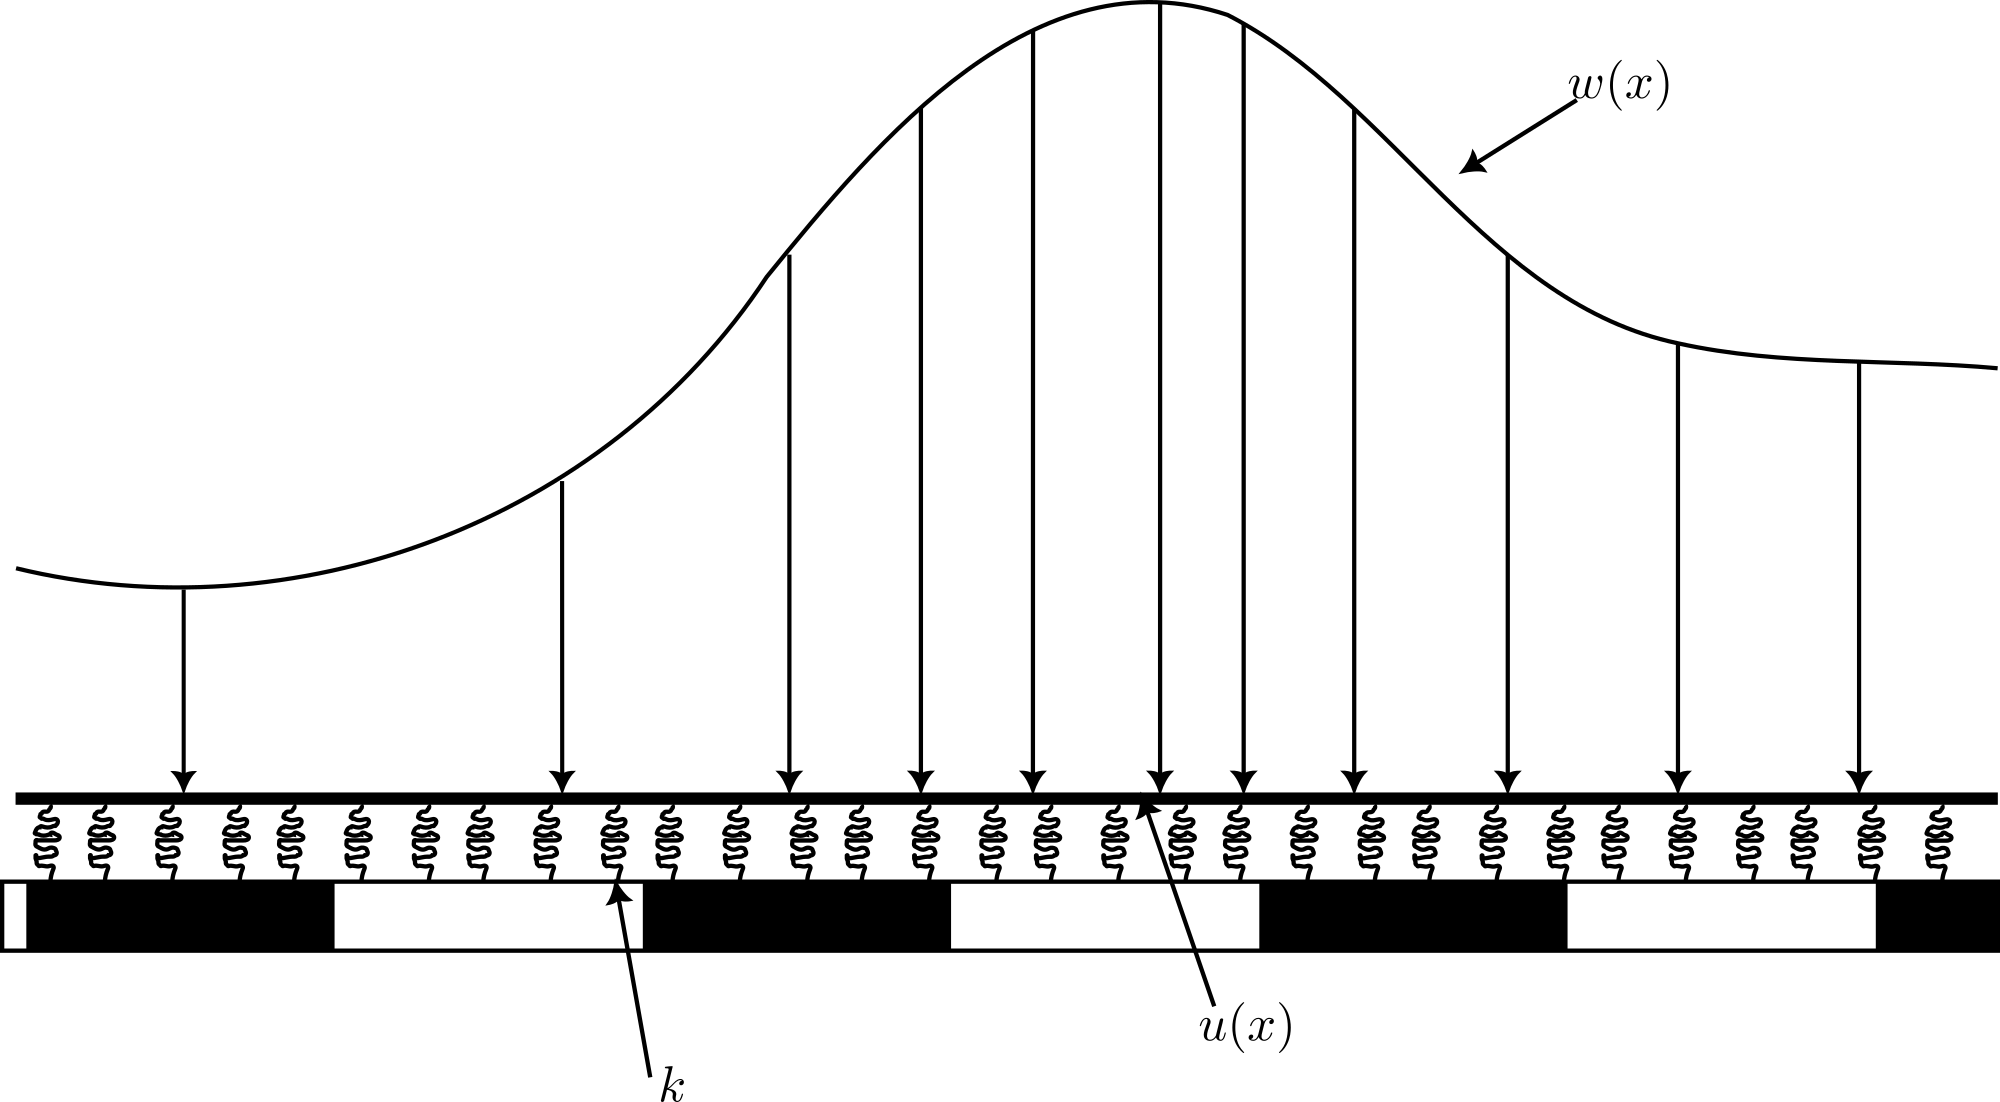
\includegraphics[width=0.75\linewidth]{include/Beam.png}
        \caption{Infinite beam on elastic foundation}
    \end{figure}

    Where the flexural rigidity of the beam, \(EI\), may be a function of \(x\), \(k\)is the spring constant per unit length. For the purposes of this example we consider both \(EI\) and \(k\) to be constant.

\subsection{Sturm-Liouville Equations}
    In this section subsection we are interested in finding the Green's function for the the general second order linear differential operator
    \begin{equation}
        L = -D^2(pD)+q
    \end{equation}
    with the general unmixed boundary conditions
    \begin{equation}
        B_1(u)=B_2(u)=0a
    \end{equation}
    where \(p\) and \(q\) are functions of the independent variable. Differential operators of this form are \df{Sturm-Liouville differential operators}. By referring to equation (\ref{eq:2OAdjoint}), it is clear that Sturm-Liouville differential operators are alwayse self adjoint since \(a=p\) and \(b=p'\). 

    For the purposes of analyzing these equations, we define the \df{conjoint}. Recall from equation (\ref{eq:2OAdjoint}) that for a second order differential operator
    \begin{equation*}
        \Lstar v = av''+(2a'-b)v'+(a''-b'+c).
    \end{equation*}
    It follows that 
    \begin{equation*}
        \intl (v\L u - u\Lstar v)dx = J(v,u)\bounds{\lima}{\limb}
    \end{equation*}
    where
    \begin{equation*}
        \begin{split}
            J(v,u) &= avu'-a'vu-av'u + bvu\\
            &=avu'- u(av)' +bvu.
        \end{split}
    \end{equation*}
    \(J(v,u)\) is the \df{conjunct} of \(v\) and \(u\).

\subsection{Example 4.4 \textit{The Generalized Green's Function}}
    As a more complex example, consider, 